\documentclass[11pt,a4paper,twocolumn]{IEEEtran}
\usepackage[utf8]{inputenc}
\usepackage{tabularx, booktabs}
\usepackage{amsmath}
\usepackage{amsfonts}
\usepackage{caption}
\usepackage{pdfpages}
\usepackage[margin=2.5cm]{geometry}
\usepackage{listings}
\usepackage{amssymb}
\usepackage{hyperref}
\usepackage{graphicx}
\usepackage{svg}

\usepackage{biblatex}
\addbibresource{bib2.bib}

\newcolumntype{L}[1]{>{\raggedright\let\newline\\\arraybackslash\hspace{0pt}}m{#1}}
\newcolumntype{C}[1]{>{\centering\let\newline\\\arraybackslash\hspace{0pt}}m{#1}}
\newcolumntype{R}[1]{>{\raggedleft\let\newline\\\arraybackslash\hspace{0pt}}m{#1}}

% \sepline dopo \maketitle rende tutto più carino
\newcommand{\sepline}{\noindent\makebox[\linewidth]{\rule{\textwidth}{1.2pt}}}
\newcommand{\bsepline}{\noindent\makebox[\linewidth]{\rule{7.5cm}{1.2pt}}}
%\newcommand{\esepline}{\noindent\makebox[\linewidth]{\rule{7.5cm}{0.5pt}}}
\newcommand{\thinsepline}{\noindent\makebox[\linewidth]{\rule{7.5cm}{0.02pt}}}
\newcommand{\thinnersepline}{\noindent\makebox[\linewidth]{\rule{7.5cm}{0.01pt}}}
\author{Monaco Saverio - 2012264 \sepline \\Neural Networks and Deep Learning - Professor: A. Testolin}
\title{{\normalsize\textsc{Università degli studi di Padova}}\vspace{-.5cm} \\ \sepline\\ \textbf{Homework \#2
\\ Unupervised Deep Learning}}

\begin{document}
	\maketitle
	\begin{abstract} As for the second homework, the main models of Unupervised Deep Learning are investigated on the FashionMNIST dataset.\\ 
	Firstly, an Autoencoder has been developed, and its hyperparameters were properly optimized. The best model has been then fine-tuned aiming for a working Classifier.\\
	As for the last model, a Generative Adversarial Network has been implemented for the task of generating new samples.
	\end{abstract}
	\section*{Data}
	FashionMNIST is a dataset of low-resolution (28$\times$28) grayscale images of fashion products from 10 categories (such as "Trousers", "Sandal", "Bag"). In the dataset there are 60,000 images for the training-set and 10,000 for the test-set.\vspace*{-.5cm}
	\begin{figure}[h]
		\centering
		\includesvg[width=0.95\linewidth]{../../1. Supervised Deep Learning/imgs/classification/fashionexamples}
		\caption{Samples of FashionMNIST}
	\end{figure}\\
	This set was used throughout all tasks of the second homework and no data augmentation was performed on it.
	\section{\textbf{Convolutional Auto-Encoders}}
	% explain autoencoders
	The task of an Auto-Encoder is to reconstruct its input image, thus it is not a Classification, nor a Regression, nor a Generative model.\\
	It consist in a Encoder, where the input images gets convoluted in a smaller space (called \textit{latent space}) and a Decoder, where the 'compressed' image gets de-convoluted to its original size.\\ The power of an Autoencoder lies in the 'bottleneck' shape (see Fig. 2). Through learning the Neural Network learns the most efficient weights and biases to reconstruct the input images as good as possible performing a dimensionality reduction.	
		\begin{figure}[h]
			\centering
			{\scriptsize
			\includesvg[width=0.95\linewidth]{../imgs/autoencoder} }
			\caption{General overview of a Convolutional Auto-Encoder}
		\end{figure}\\
	Convolutional Auto-encoder are used mainly for \textit{anomaly detection}, and \textit{denoising}.
		\subsection{\textbf{Methods}}
		% describe your model architectures and hyperparameters
		The Autoencoder was implemented through a Pyhton class using \textit{Pytorch} for building the layers. The only free parameter for the initialization is the size of the \textit{latent space} dimension, while the activation was kept fixed to ReLU.\medskip\\
		\textbf{Encoder:}
		\begin{itemize}
			\item First Convolutional layer: in\_channels=1, out\_channels=8, kernel\_size=3;
			\item Second Convolutional layer: in\_channels=8, out\_channels=16, kernel\_size=3;
			\item Third Convolutional layer: in\_channels=16, out\_channels=32, kernel\_size=3;
			\item First Linear layer: in\_features=3*3*32, out\_features=64;
			\item Second Linear layer: in\_features=64, out\_features=latent\_dim;
		\end{itemize}
		\textbf{Decoder:} is a specular Network of the Encoder built with the use of \texttt{nn.ConvTranspose2d} for the de-convolution.\\
		The Mean Square error Loss was adoperated to evaluate the models, hence the difference squared of each pixel of the real image and its reconstructed was computed.
		\subsection{\textbf{Results}}
		%  present the simulation results
		Firstly, a 2-Dimensional latent space Autoencoder was trained for inspecting the points of the testing images in the Latent Space (that can be plotted as a matter of fact as a 2D scatter plot):\vspace*{-.5cm}
		\begin{figure}[h]
			\centering
			\hspace*{-1.3cm}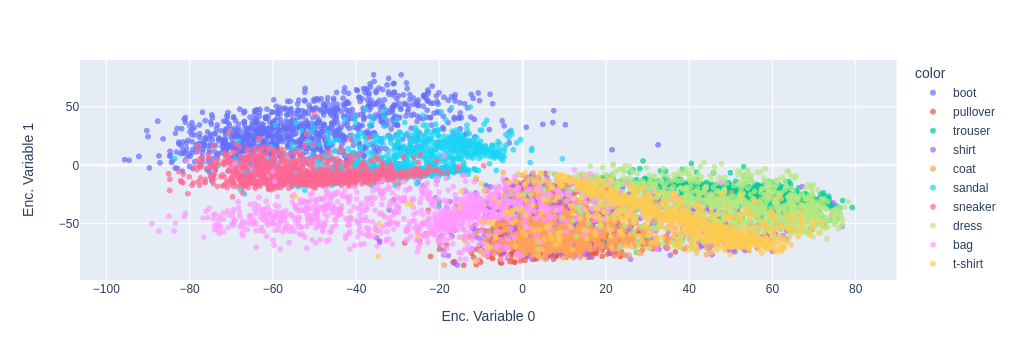
\includegraphics[width=1.2\linewidth]{../imgs/newplot}
			\caption{Latent space of Autoencoder}
			\label{fig:2dlatent}
		\end{figure}\\
		Each dot represents the coordinate of a single image of the test dataset in the 2-D latent space, and its color represents its label (that was never given to the Network).\\
		Without ever given the information of the label to the network, it grouped each dot according to it, in addition, dots of different class that are close in the latent space, can be considered semantically close, so it can be defined a metric in the \textit{latent space} on how much clothes look alike.\\
		To demonstrate better the last statement, dots along a line that connects the blue path and the red path were decoded (namely from the "Boot" group to the "Sneaker" group):\vspace*{-.5cm}
		\begin{figure}[h]
			\centering
			\includesvg[width=1\linewidth]{../imgs/autoencoder_transf}
			\vspace*{-1cm} %dont ask me why
			\caption{Gradual transformation of a Boot to a Sneaker}
			\label{fig:trasf}
		\end{figure}\medskip\\
		After the inspeciton of the latent space, a Grid Search was performed using Optuna Python library for hyperparameters optimization. The dimension of the encoded space this time was kept fixed to 16, while the initial learning rate, regularization term of the optimizer, and the optimizer itself were tunable:
		\begin{itemize}
			\item[-] Optimizer: Adam, SGD;
			\item[-] Initial Learning rate: from 1e-4 to 1e-3;
			\item[-] Regularization term: from 1e-5 to 1e-3;
		\end{itemize}
		\thinsepline\\
		\textbf{Best model:}
		\begin{itemize}
			\item Optimizer: Adam;
			\item Learning Rate: 0.00099
			\item Regularization: 3.5237e-5
		\end{itemize}
		\thinnersepline\\
		Epochs: 60\\
		MSE on Test Set: 0.017237\\
		\thinsepline\\
		\begin{figure}[h]
			\centering
			\includesvg[width=1\linewidth]{../imgs/bestautoencoder_recprog}
			\caption{Performance of Autoencoder during its learning process}
			\label{fig:recproc}
		\end{figure}\\
	The Model seems to properly reconstruct the shape of the input image, however, it does not seems to learn during its training how bright a certain pixel must be. 
	\section{\textbf{Fine-tuning an Autoencoder}}
	% explain gans
	With some modifications to the model, autoencoders can perform the classification task. In order to achieve this, we can place on top of the encoder a fully connected neural network and completely remove the decoder part. If the layers of the encoder are frozen, the task of classificating the images will actually be a task of classificating the points in the encoded space to their labels.
	\subsection{\textbf{Methods}}
	% describe your model architectures and hyperparameters
	The structure of the fine-tuned autoencoder is:\\
	\textbf{Encoder:} same as in the previous section, weights and biases frozen.\\
	\textbf{Fully Connected Neural Network:}
	\begin{itemize}
		\item First Linear Layer:\\ input\_features=latent\_dim,\\ output\_features=256;
		\item Second Linear Layer: input\_features=256, output\_features=256;
		\item Third Linear Layer: input\_features=256, output\_features=128;
		\item Last Linear Layer: input\_features=128, output\_features=10;
	\end{itemize}
	Between each layer ReLU activation function was chosen and as last activation LogSoftmax was applied.\bigskip\\

	\subsection{\textbf{Results}}
	%  present the simulation results
	\thinsepline\\
	\textbf{Fine-Tuned Autoencoder:}
	\begin{itemize}
		\item Loss Function: Cross Entropy Loss 
		\item Optimizer: Adam;
		\item Learning Rate: 2e-4
		\item Regularization: 1e-5
	\end{itemize}
	\thinnersepline\\
	Epochs: 100\\
	Accuracy on Test Set: 83.49 \% \\
	\thinsepline\vspace*{-1cm}\\
	\begin{figure}[h]
		\centering
		\includesvg[width=1\linewidth]{../imgs/ftuner_heatmap}
		\caption{Confusion matrix of the model on the test dataset}
		\label{fig:heatmap} % 87.69 %
	\end{figure}\\
	Compared to the dedicated Convolutional Network from Homework 1, the accuracy is slightly lower. However, with the hypothesis of having an already well trained autoencoder, transfer learning results in faster learning times.
		
	\section{\textbf{Generative Adversarial Networks}}
	% explain gans
		The last model chosen for the generative task was the Generative Adversarial Network (GAN). A GAN is really two Neural Networks, the Generator that tries to imitate the input dataset, and the Discriminator that trie to tell the difference betweent the fake images from the generator and the real images of the dataset.\\
		At the beginning of lerning, the discriminator always does a good job in detecting what images are fake, since the generator will output images close to random noise, but eventually the generator picks up until ideally the discriminator does not distinguish a fake image from a real one.
		\subsection{\textbf{Methods}}
		% describe your model architectures and hyperparameters
		The GAN was implemented through a single Python class, containing both models for discriminating and generating:\\
		\textbf{Discriminator:}
		\begin{itemize}
			\item First Linear Layer: \\input\_features=28$\times$28,\\ output\_features=hidden\_size;
			\item Second Linear Layer: \\input\_features=hidden\_size,\\ output\_features=hidden\_size;
			\item Third Linear Layer: \\input\_features=hidden\_size,\\ output\_features=1;
		\end{itemize}
		For the Discriminator network, LeakyReLU activation was chosen between eachlayer and Sigmoid for the last.\\
		\textbf{Generator:}
		\begin{itemize}
			\item First Linear Layer:\\ input\_features=latent\_size,\\ output\_features=hidden\_size;
			\item Second Linear Layer:\\ input\_features=hidden\_size,\\ output\_features=hidden\_size;
			\item Third Linear Layer:\\ input\_features=hidden\_size,\\ output\_features=28$\times$28;
		\end{itemize}
		For the Generator network, between each layer ReLU was chosen as activation function and Tanh as last activation.\medskip\\
		The free parameters for the initialization of the GAN are \texttt{hidden\_size} that determines the size of the hidden layers on both networks and \texttt{latent\_size} that is the size of the random input image for the generator.
		\subsection{\textbf{Results}}
		%  present the simulation results
		Due to the extremely long periods of time for the training of a GAN, no Grid Search was adopted.
		\thinsepline\\
		\textbf{Parameters of the GAN:}
		\begin{itemize}
			\item latent\_size = 100
			\item hidden\_size = 784
			\item Epochs = 300
			\item Learning Rate = 1e-4
		\end{itemize}
		\thinsepline\newpage
		\begin{figure}[h]
			\centering
			\includesvg[width=.85\linewidth]{../imgs/ganlosses}
			\caption{Losses of Discriminator and Generator Networks}
			\label{fig:ganloss}
		\end{figure}
	During training, samples of generated images were stored:
	\begin{figure}[h]
		\centering
		\includesvg[width=1\linewidth]{../imgs/gan0}\vspace*{-.7cm}\\
		%\includesvg[width=1\linewidth]{../imgs/gan50}\\
		\includesvg[width=1\linewidth]{../imgs/gan100}\vspace*{-.7cm}\\
		%\includesvg[width=1\linewidth]{../imgs/gan150}\\
		%\includesvg[width=1\linewidth]{../imgs/gan200}\\
		\includesvg[width=1\linewidth]{../imgs/gan250}\vspace*{-.5cm}\\
		\caption{Fake generated samples}
		\label{fig:ganimgs}
	\end{figure}
	In some images it is possible to see that the generator tries to output multiple clothes at once although it becomes less common with further training.\\
	The generated data appear \textit{noisy}, coincidentally Autoencoders can denoise images, the following images were generated through the GAN and then fowarded through the Autoencoder found using Optuna:
	\begin{figure}[h]
		\centering
		\includesvg[width=1\linewidth]{../imgs/genandfil_0}\vspace*{-.5cm}\\
		\includesvg[width=1\linewidth]{../imgs/genandfil_1}\vspace*{-.5cm}\\
		\includesvg[width=1\linewidth]{../imgs/genandfil_2}\vspace*{-.5cm}\\
		\includesvg[width=1\linewidth]{../imgs/genandfil_3}\vspace*{-.5cm}\\
		\includesvg[width=1\linewidth]{../imgs/genandfil_4}\vspace*{-.5cm}\\
		\caption{Generated and filtered images}
		\label{fig:filter}
	\end{figure}\\
	Although being a questionable choice, the combination GAN+Autoencoder generates new samples that are quite satisfying and for some of them, may fool a human aswell.
	\newpage
	\onecolumn
	\section{\textbf{Appendix}}
	
		\subsection{Hyperparameter optimization using Optuna}
		\begin{figure}[h]
			\centering
			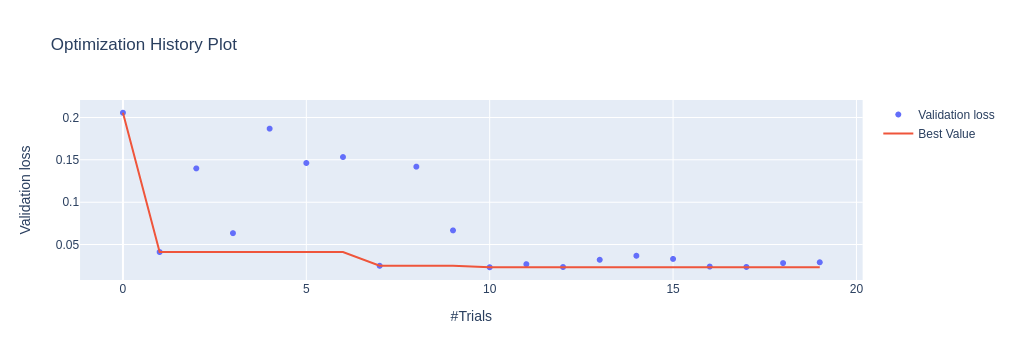
\includegraphics[width=1\linewidth]{../imgs/newplot(2)}
			\caption{Best model through trials}
			\label{fig:newplot2}
		\end{figure}
	\begin{figure}[h]
		\centering
		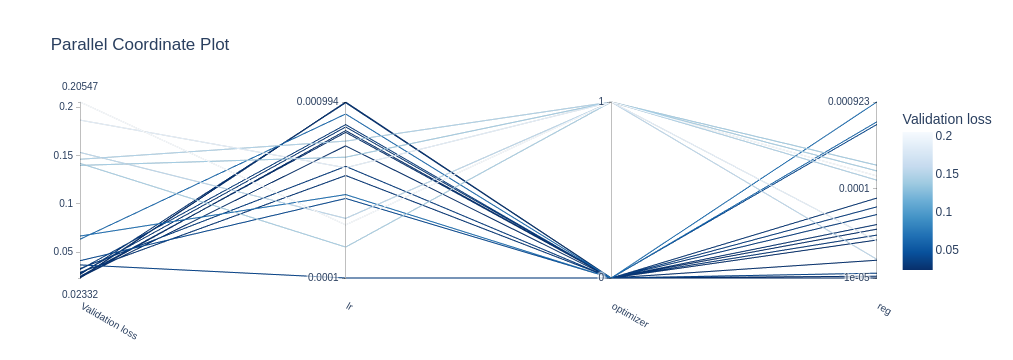
\includegraphics[width=1\linewidth]{../imgs/newplot(3)}
		\caption{Overview of parameter combinations and their Validation loss}
		\label{fig:newplot3}
	\end{figure}\newpage
	\subsection{Latent space of Trained and Untrained Network}
		\begin{figure}[h]
			\centering
			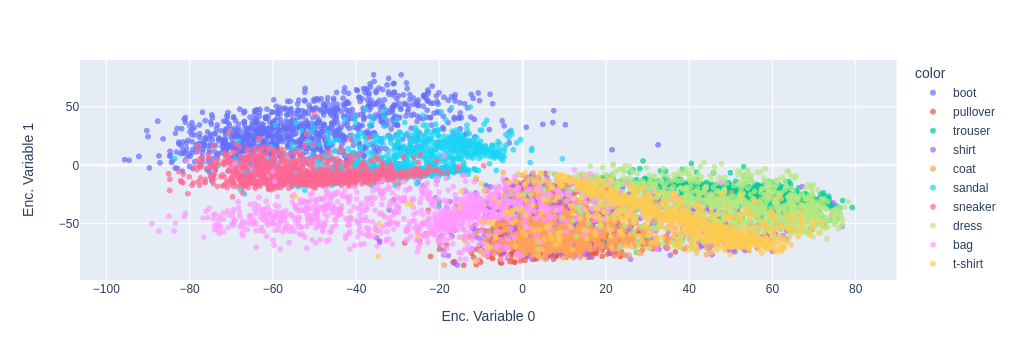
\includegraphics[width=1\linewidth]{../imgs/newplot}
			\caption{Latent space of 2-D Trained Autoencoder}
			\label{fig:lspace_tr}
		\end{figure}
		\begin{figure}[h]
			\centering
			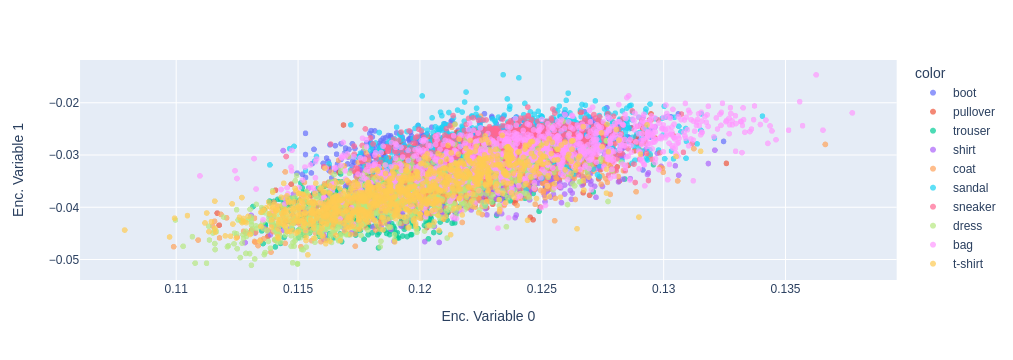
\includegraphics[width=1\linewidth]{../imgs/newplot(1)}
			\caption{Latent space of 2-D \textbf{Un}trained Autoencoder}
			\label{fig:lspace_un}
		\end{figure}
	Fig.\ref{fig:lspace_tr} and Fig.\ref{fig:lspace_un} shows respectively the encoded vectors of the images from the test set in latent space of the Trained and the Untrained Autoencoder with latent space dimension equal to 2. The colors of the dots were added separately and represent the class each point belongs to.\\
	The dots in the encoded space of the untrained network are focused randomly in a small neighborhood around zero, while for he trained net, they are more sparsed and each classes are almost separated one another.
	\newpage
	 \subsection{PCA and t-SNE on Latent Space}
	 \begin{figure}[h]
	 	\centering
	 	\includesvg[width=.8\linewidth]{../imgs/lats_pca}
	 	\caption{PCA over 16-dimensional latent space autoencoder}
	 	\label{fig:psa}
	 \end{figure}
	 \begin{figure}[h]
	 	\centering
	 	\includesvg[width=.8\linewidth]{../imgs/lats_tsne}
	 	\caption{TSNE over 16-dimensional latent space autoencoder}
	 	\label{fig:tsne}
	 \end{figure}\newpage
\end{document}